\section{Components}

With basis in our system definition in chapter \ref{abc} and our evaluation of criteria in section \ref{sec:criteria} we found that our main priority is flexibility. To obtain high flexibility we created a closed-strict layers component architecture, we did this to avoid complex dependencies between components and therefore making it easy to change an interface, a function component, or . 
The architecture has three layers: User- and System-interfaces, Functions, Model as shown on figure \ref{fig:SystemComponent}. The figures components will be explained in section \ref{sub:SystemComponent} 

\begin{figure}[]
	\centering
		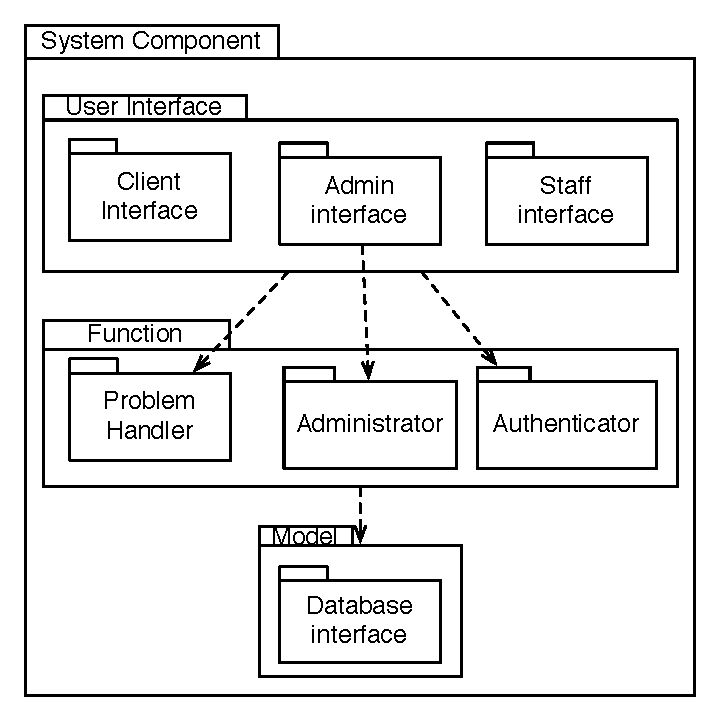
\includegraphics[scale=0.5]{input/architectural_design/system_component_denvibruger.pdf}
	\morscaption{Our system component}
	\label{fig:SystemComponent}
\end{figure}


\subsection{System Component}
\label{sub:SystemComponent}

\paragraph{\cinterface}
The client interface get inputs from the client, through this interface the client submits problems, post comments and search for existing problems.
The functions associated with this interface are located in the Problem Handler component.  

\paragraph{\sinterface}
Through this interface the staff members can access all the client functions, submit solutions, post comments to \open[] problems, view \worklist[] and administrate problems.
This Interface uses the Problem Handler component. 

\paragraph{\ainterface}  
\fixme{kim: hvad kan man i admin mode?}
The interface has access to all the \aclient[] functions, the \astaff[] functions, tags/category management, department management and administration of the client/staff. This is due to the fact that if a person is an \admin[], then he/she also is a \astaff[] and a \aclient[]. The Admin Interface uses the Problems Handler and the Administrator component. 

\paragraph{Problem Handler}
The problem handler component controls the handling of new problems, the handling of solutions, the searching function, recording and sending statistics, manages comments and sending notifications by using the notifier component.
This component is also responsible for sending out signals to relevant actors. e.g. if a user posts a comment the relevant staff member(s) receives a notification.  

\paragraph{Administrator}
Through the admin interface the admin component can be accessed. The functions affiliated with this component are control of departments, management of tags/categories and adding/removing of staffs and clients.   

\paragraph{Authenticator}
To determine which rights a person have, they have to authenticate them selves as either client or staff/admin, this occurs through an authenticator component which communicates with the database interface. \fixme{kim: skældner autheticator mellem staff og admin?}  

\paragraph{Database Interface}
The database interface receives all database requests and translate them to the correct database language.

\subsection{}
beskrivelse af hvordan system component virker.

beskrivelse af hvordan det alternative virker og hvorfor vi bruger den.

\paragraph{Login System Interface}
\fixme{kim: skal skrives, (skal det være et system Interface eller userinterface?)}


\begin{figure}[]
	\centering
	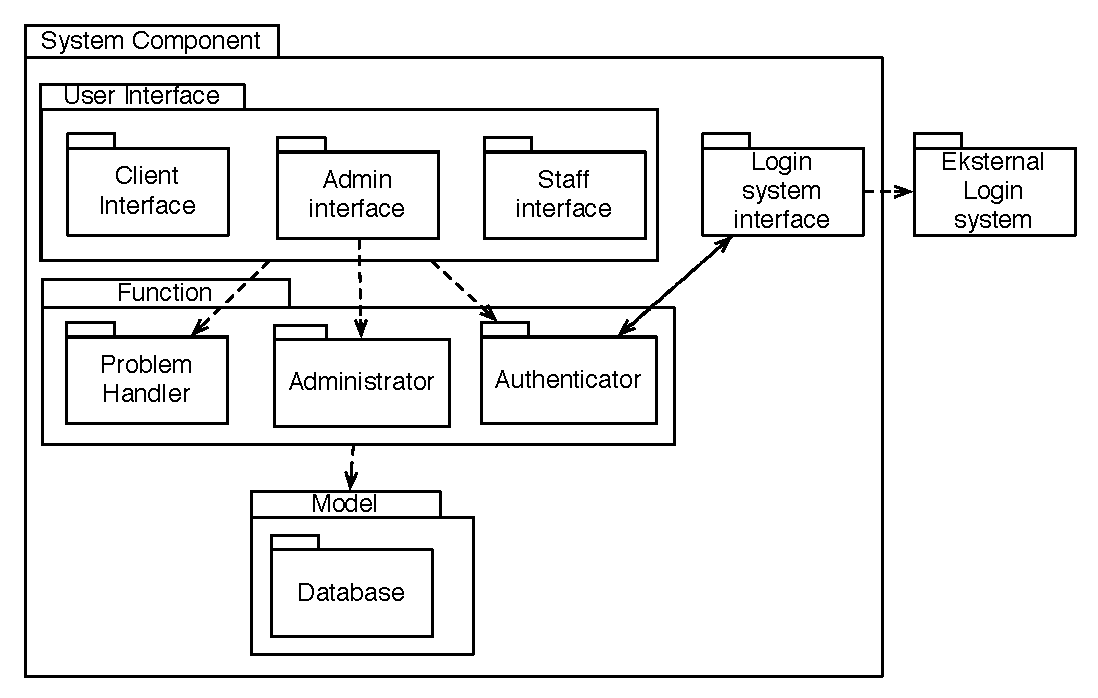
\includegraphics[scale=0.5]{input/architectural_design/system_component_denalternative.pdf}
	\morscaption{}
	\label{fig:SystemComponent}
\end{figure}


\subsection{Client-Server}
Because we are designing a help desk, we are dealing with users who are not present in a specific location. Therefore we also designed the system using a client-server architecture.
On the client side there is a user interface and on the server side the functionality and model are located. By using Local Presentation~\cite{roedeaalborg}[p.~200] we enable clients to access the system from anywhere, and still keep the functionality and model on the server and thus keeping the system flexible.         
\fixme{kim: lave evt et billede med serverclient}

\begin{figure}%
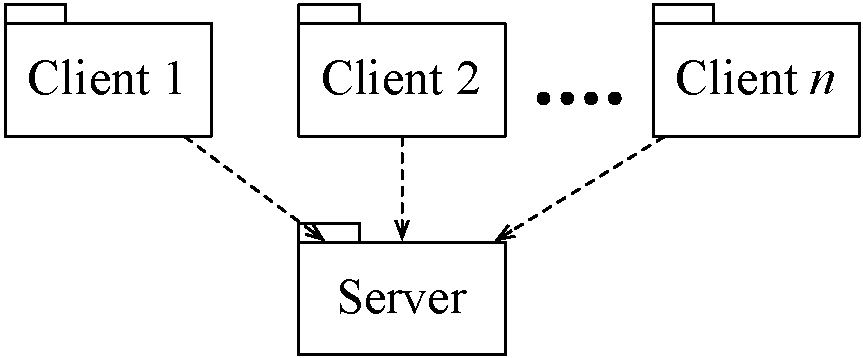
\includegraphics[scale=0.5]{input/architectural_design/client-server-architecture-pattern.pdf}%
\caption{}%
\label{}%
\end{figure}